\documentclass[11pt, a4paper]{report}
\usepackage[francais]{babel}
\usepackage{dirtytalk}
\usepackage{amsmath}
\usepackage{todonotes}
\usepackage{tabularx}
\usepackage{listings}
\definecolor{codegreen}{rgb}{0,0.6,0}
\definecolor{codegray}{rgb}{0.5,0.5,0.5}
\definecolor{codepurple}{rgb}{0.58,0,0.82}
\definecolor{backcolour}{rgb}{0.95,0.95,0.92}

\lstdefinestyle{mystyle}{
    backgroundcolor=\color{backcolour},   
    commentstyle=\color{codegreen},
    keywordstyle=\color{magenta},
    numberstyle=\tiny\color{codegray},
    stringstyle=\color{codepurple},
    basicstyle=\ttfamily\footnotesize,
    breakatwhitespace=false,         
    breaklines=true,                 
    captionpos=b,                    
    keepspaces=true,                 
    numbers=left,                    
    numbersep=5pt,                  
    showspaces=false,                
    showstringspaces=false,
    showtabs=false,                  
    tabsize=2
}
\lstset{style=mystyle}
\lstset{
  language=Python,
  inputencoding=utf8/latin, % or utf8
  commentstyle=\itshape\color{gray} % Adjust the comment style
}

\newcommand{\TALN}{traitement automatique du langage naturel}

\title{Traitement automatique du langage naturel \newline
(avant deep learning)}
\author{Václav Gregor}
\date{\today}
\newtheorem{hyp}{Hyp}[section]

\begin{document}

\maketitle

\tableofcontents


\begin{abstract}
  Ces notes présentent un regard épistémologique sur le domaine du traitement automatique du 
  langage naturel. Elles parlent de son histoire et de son développement.
\end{abstract}


\chapter{Introduction}
  Nous allons en premier regarder l'histoire du traitement automatique du langage 
  naturel (TALN en abrégé), en passant par ses 
  trois approches principales : symbolique, statistique et neuronale. 
  Il est impossible pour moi de donner un résumé complet de l'histoire de ce domaine, 
  ainsi que de décrire chaque approche parfaitement. J'ai donc pris la décision 
  d'utiliser des exemples de programmes, d'expériences et de modèles spécifiques 
  pour illustrer le développement du TALN. 
  
  Dans le deuxième chapitre, on se concentra sur le word embedding : la représentation 
  des mots par des vecteurs. On expliquera les motivations de cette technique, son fonctionnement ses les 
  applications. 
\chapter{Brève histoire du TALN}
  \section{Approche symbolique}
    \subsection{l'expérience Georgetown-IBM}
    \cite{wikipedia-nlp}
    \cite{wikipedia-georgetown} 
    \cite{hutchins-georgetown}
Le domaine a débuté dans les années 1950. Le premier résultat 
marquant et connu par le public général était l'expérience Georgetown-IBM en 1954. Il s'agissait d'une 
démonstration de traduction automatique du russe vers l'anglais, comme le 
contexte historique le voulait.

Le programme contenait 6 règles de grammaire, un vocabulaire de 250 éléments lexicaux 
(thèmes et désinences des mots compris), et était capable de traduire 60 
phrases. Les phrases parlaient surtout de la chimie, les mathématiques, la 
communication, la métallurgie et les affaires militaires. Il est essentiel de 
noter que les phrases ont été choisies soigneusement par les auteurs du programme. 
Certaines règles et opérations du programme était spécifiques à un nombre limité 
de mots et de phrases d'entrée. Chaque mot russe du vocabulaire correspondait à un ou deux 
équivalents anglais. En plus, chaque mot avait 3 codes numériques associés, qui 
déterminaient la règle de grammaire à utiliser pour produire la sortie. 
Si cette description nous rappelle la notion de 
"hardcoding", ce n'est pas par hasard. Le programme était essentiellement un 
dictionnaire assez limité, qui cherchait la traduction correspondante pour chaque 
mot russe, et qui appliquait l'une des 6 règles pour rendre la phrase anglaise 
à la sortie plus correcte. Regardons ceci sur un exemple. 

\noindent \textbf{La phrase russe (en alphabet latin)} \newline 
Vyelyichyina ugla opryedyelyayetsya otnoshyenyiyem dlyini dugi k radyiusu. \newline  
\textbf{Traduction française} \newline 
L'ampleur de l'angle est déterminée par la relation entre la longueur de l'arc et le rayon. \newline 
\textbf{Traduction anglaise obtenue par le programme} \newline 
Magnitude of angle is determined by the relation of length of arc to radius.

Regardons maintenant les informations que le programme avait à sa disposition pour traduire 
cette phrase. 

\begin{table}[h] % "h" specifies the placement of the table (here: "here")
  \centering % Centers the table horizontally
  \begin{tabular}{|c|c|c|c|c|c|} % Specifies the format of the table (here: two centered columns with vertical lines)
    \hline % Horizontal line
    entrée russe & équivalents anglais & code 1 & code 2 & code 3 & règle \\ % Table content separated by "&", "\\" starts a new row
    \hline
    vyelyichyina & magnitude & *** & *** & ** & 6 \\
    \hline
    ugl- & coal, angle & 121 & *** & 25 & 2 \\
    \hline 
    -a & of & 131 & 222 & 25 & 2 \\
    \hline 
    opryedyelyayetsya & is determined & *** & *** & ** & 6 \\
    \hline 
    otnoshyenyi- & relation, the relation & 151 & *** & ** & 5 \\ 
    \hline 
    -yem & by & 131 & *** & ** & 3 \\ 
    \hline 
    dlyin- & length & *** & *** & ** & 6 \\ 
    \hline 
    -i & of & 131 & *** & 25 & 3 \\ 
    \hline 
    dug- & arc & *** & *** & ** & 6 \\
    \hline 
    -yi & of & 131 & *** & 25 & 3 \\ 
    \hline 
    k & to, for & 121 & *** & 23 & 2 \\ 
    \hline 
    radyius- & radius & *** & 221 & ** & 6 \\ 
    \hline 
    -u & to & 131 & *** & ** & 3 \\
    \hline
  \end{tabular}
  \caption{Exemple de traduction (Georgetown-IBM)} % Caption for the table
  \label{tab:example} % Label for referencing the table
\end{table}

Le premier mot (vyelyichyina) n'a qu'un seul équivalent anglais (magnitude) et son 
premier code étant vide (***) infère la règle 6 : la traduction est simplement copiée 
à la sortie. \newline 
\textit{sortie partielle : magnitude} 

Le deuxième mot (ugla) est séparé en thème (ugl-) et désinence (-a). 
Le thème (ugl-) appelle la règle 2 avec son code 1 (121). La règle 2 va chercher à trouver 221 ou 222 
comme le code 1 de la prochaine entrée (-a). On trouve 222 pour le code 1 de l'entrée 
"-a", et donc on choisit le deuxième équivalent de "ugl-" pour la sortie (angle). \newline 
\textit{sortie partielle : magnitude angle}

L'entrée suivante (-a) appelle la règle 3 avec son code 1 (131). Cette règle va regarder si le 
code 2 de l'entrée précédente est égal à 23. Comme ce code est vide (***), on sélectionne le seul 
équivalent de "-a" et on inverse l'ordre des deux mots (ce qui produit "of angle"). \newline
\textit{sortie partielle : magnitude of angle}

\begin{figure}[t]
  \centering
  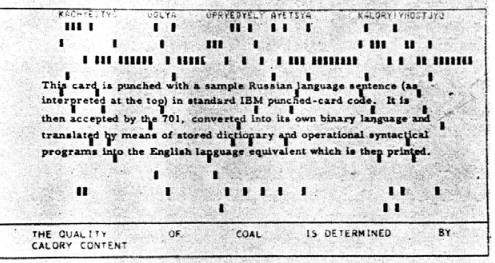
\includegraphics[width=1\textwidth]{punched-card.png}
  \caption{Une carte perforée utilisée dans l'expérience.}
  \label{fig:carte-perforee}
\end{figure}

\begin{figure}[t]
  \centering
  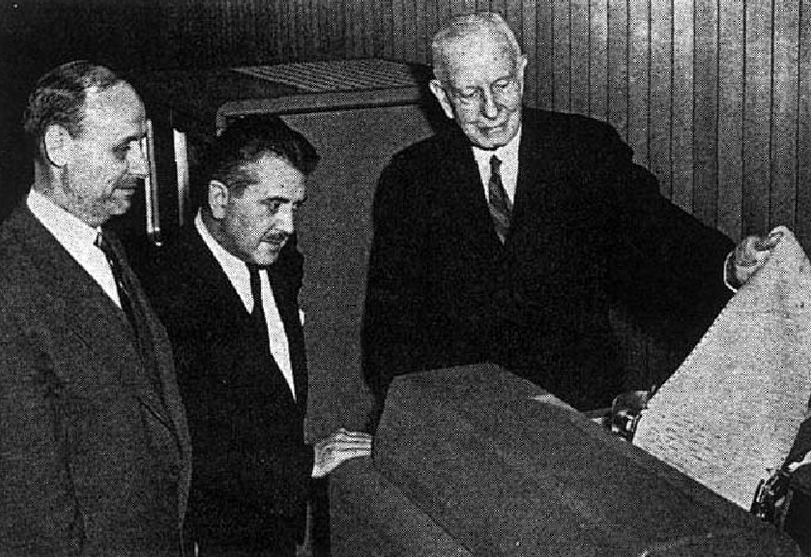
\includegraphics[width=1\textwidth]{georgetown-chercheurs.png}
  \caption{Hurd (directeur de la division des sciences appliquées de IBM), Dostert (traducteur franco-américain) et Watson (fondateur d'IBM) lors de la démonstration.}
  \label{fig:carte-perforee}
\end{figure}

Le reste de la traduction serait trouvé similairement, on va donc s'arrêter ici. Je pense que ce 
petit exemple est suffisant pour illustrer le fait que le programme ne fait que suivre bêtement les 
règles "hardcodées" par les chercheurs. Avant d'être programmé, ce processus qu'on vient d'essayer 
a été testé par des personnes avec aucune connaissance en russe, pour vérifier qu'il produit des 
résultats corrects sur les phrases données. Si on essaie de trouver une analogie, on peut imaginer
qu'on donne un dictionnaire russe-anglais à une personne anglophone qui ne parle pas russe, on lui demande 
de traduire des phrases, mais en plus de ça, on lui donne aussi une liste d'instructions à suivre 
pour produire des phrases plus naturelles (en n'utilisant que le dictionnaire pour traduire). 

En gros, la valeur de l'expérience Georgetown-IBM repose dans l'analyse de la grammaire russe et dans 
l'invention des 6 règles qui permettent de traduire les phrases prédéterminées sans aucune réflexion. 
Cette tâche a ensuite été passée à un ordinateur. 

Ce qui est intéressant, c'est que cette expérience était vue comme un énorme succès. Voici quelques 
extraits d'articles de journaux américains contemporains pour illustrer ce point.
\begin{quote} 
It is expected by IBM and Georgetown University, which collaborated on this project,
that within a few years there will be a number of “brains” translating all languages
with equal aplomb and dispatch. (Kenny, Christian Science Monitor)
\end{quote}

\begin{quote}
The girl who operated 701 did not understand a word of Soviet speech and yet more
than 60 Soviet sentences were given to the “brain” which translated smoothly at the
rate of about 2.5 lines a second. (Kenny, Christian Science Monitor)
\end{quote}

\begin{quote}
The “brain” didn’t even strain its superlative versatility and flicked out its
interpretation with a nonchalant attitude of assumed intellectual achievement. (Kenny,
Christian Science Monitor)
\end{quote}

On remarque surtout l'utilisation du mot "brain", alors que le programme n'était qu'une suite 
de branchements IF ELSE. Une jolie illustration du fait que dans les années 1950, les ordinateurs 
étaient vus comme des cerveaux mystérieux par une partie significative de la population. 
Ceci a permis à cette démonstration d'arriver à son but : attirer l'attention du public et du 
gouvernement américain et obtenir des financement pour 
la recherche future dans ce domaine. 
  
    \subsection{ELIZA}
    \cite{wikipedia-eliza}
    \cite{eliza-original}
    \cite{eliza-gpt}
    \cite{weizenbaum-book}
    \cite{weizenbaum-pic}
      \subsubsection{Introduction}
En 1966, ELIZA est créé par Joseph Weizenbaum - un programme pour explorer l'interaction entre les humains et 
les machines. ELIZA est capable d'utiliser les règles définies dans un script externe pour 
simuler une conversation. Le programme repose sur l'application du pattern-matching et d'une 
méthodologie de substitution, qui seront expliqués sur un exemple.
Son script le plus célèbre : DOCTOR, simule un psychothérapeute de l'école Rogérienne
("Rogerian school" en anglais). Ce qui est important à retenir est que dans cette approche 
psychothérapeutique, le psychologue répète souvent les paroles du patient à ce dernier. 
Ce script permet donc à ELIZA de garder l'illusion d'une conversation avec un humain, 
sans rien savoir du monde réel. Citons Weizenbaum qui explique ce point:

\begin{quote}
  This mode of conversation was chosen because the psychiatric interview is one of the 
  few examples of categorized dyadic natural 
  language communication in which one of the participating pair is free to assume the pose 
  of knowing almost nothing of the real world. If, for example, one were to tell a 
  psychiatrist "I went for a long boat ride" and he responded "Tell me about boats", 
  one would not assume that he knew nothing about boats, but that he had some purpose 
  in so directing the subsequent conversation. It is important to note that this 
  assumption is one made by the speaker. \cite[L'article original de Joseph Weizenbaum
  sur ELIZA]{eliza-original}
\end{quote}

      \subsubsection{Fonctionnement général}
Le fonctionnement général d'ELIZA peut être décrit ainsi : le texte entré par l'utilisateur 
est inspecté pour y trouver l'un des "mots-clés. Si un mot-clé est trouvé, l'entrée est transformée 
en appliquant une règle associée avec ce mot-clé. Si aucun mot-clé n'est trouvé, une réponse générale 
ne dépendant que de l'entrée est formulée, ou bien une transformation déjà utilisée 
avant est appliquée. 
Les mots-clés et leurs transformations sont définis dans le script externe. 
ELIZA peut donc travailler 
avec n'importe quel script, et c'est ce dernier qui détermine sa "personnalité". 

Weizenbaum résume ceci en 5 problèmes techniques :
\begin{itemize}
  \item L'identification du mot-clé le plus important, car il peut y en avoir plusieurs dans une 
  seule entrée.
  \item L'identification d'un contexte minimal dans lequel le mot-clé apparaît. Par exemple, si le 
  mot-clé est "you", est-ce qu'il est suivi par "are" ? Dans ce cas, une assertion sur ELIZA est 
  probablement faite par l'utilisateur. Une telle information peut nous aider avec le choix de transformation.
  \item Le choix d'une transformation appropriée et l'exécution de cette transformation. 
  \item Un mécanisme qui permettra à ELIZA de répondre d'une façon "intelligente" si 
  aucun mot-clé est trouvé. 
  \item Un mécanisme pour faciliter l'édition et extension d'un script. Ce point nous intéressera peu, 
  car il n'est pas essentiel pour comprendre le fonctionnement d'ELIZA. 
\end{itemize}

      \subsubsection{Les transformations}
Le principe des transformation est expliqué très bien par Weizenbaum dans son article original (ce qui suit 
en est une analogie) : 
considérons la phrase "Je suis très malheureux". Supposons qu'un étranger (pourquoi pas un Slovaque) avec un niveau de 
français limité a entendu cette phrase mais n'a compris que le début de la phrase : "Je suis". 
Le Slovaque a quand même retenu le reste de la phrase, mais il ne sait pas ce qu'il veut dire. 
Souhaitant répondre à la personne, il remplace "Je suis" par "Ca fait longtemps que tu es"
et ensuite il répète le reste de la phrase originale pour formuler sa réponse :
"Ca fait longtemps que tu es malheureux ?". Le Slovaque a appliqué un certain modèle
à la phrase originale, qui l'a séparée en deux parties : "Je suis" et "très malheureux".
Il a ensuite utilisé une transformation qui lui a permis de répondre même s'il ne comprenait pas 
la phrase entière. Cette transformation lui dit qu'à toute phrase de la forme 
"Je suis BLABLA", il est possible de répondre avec "Ca fait longtemps que tu es BLABLA ?", 
sans savoir ce que le BLABLA veut dire. Voilà ce que fait ELIZA.  

      \subsubsection{Décomposition et réassemblage}
Plus formellement, considérons la phrase "It seems that you hate me". On l'a décompose ainsi
en quatre parties :

  \begin{center}
    (1)It seems that (2)you (3)hate (4)me
  \end{center} 
  
  Supposons que l'étranger ne comprend que les parties 2 et 4 de cette phrase. Les mots qu'il a compris 
  représente le/-s-mot/-s clé pour ELIZA. Ici, il s'agit des mots "you" et "me". Une façon générale 
  pour lui de répondre pourrait être "What makes you think I hate you?". C'est-à-dire il jette la partie (1), 
  il traduit les parties qu'il a compris - "you" devient "I" et "me" devient "you" et finalement il 
  ajoute une phrase de base "What makes you think" devant tout ça. 

  On peut alors représenter la règle de décomposition que l'étranger a utilisée plus formellement :

  \begin{center}
    (0 YOU 0 ME)
  \end{center} 

  où le 0 correspond à un nombre quelconque de mots dans la phrase originale. 
  Voici la règle de réassemblage correspondante.

  \begin{center}
    (WHAT MAKES YOU THINK I 3 YOU)
  \end{center} 
  
  où le 3 correspond à la troisième partie de la décomposition de la phrase originale 
  - ce qui se trouve entre les seuls mots compris "you" et "me". 
   
  Si on prend la phrase "It seems that you hate", la règle de décomposition 
  (0 YOU 0 ME) échoue, comme on n'arrive pas à trouver le mot "ME". On voit donc le 
  besoin d'avoir plusieurs décompositions pour un seul mot-clé, qui vont être testées 
  une par une sur la phrase d'entrée. En plus, on aura plusieurs réassemblages possibles pour 
  chaque décomposition. On peut alors représenter les données correspondantes à un mot-clé 
  ainsi : 

  \begin{align*}
    \left\{ K: \right. 
    &\left[ D_{1}, R_{1, 1}, R_{1, 2} \ldots R_{1, m_{1}} \right], \\
    &\left[ D_{2}, R_{2, 1}, R_{2, 2} \ldots R_{2, m_{2}} \right], \\
    &\ldots \\
    &\left. \left[ D_{n}, R_{n, 1}, R_{n, 2} \ldots R_{n, m_{n}} \right] \right\}
  \end{align*}

  où à un mot-clé $K$, on associe $n$ règles de décomposition $D_{1} \ldots D_{n}$, et à 
  chaque règle de décomposition $D_{i}$ on associe $m_{i}$ règles de réassemblage 
  $R_{1} \ldots R_{m_{i}}$. Un script pour ELIZA 
  n'est alors qu'une liste de telles structures. Un dictionnaire qui a comme clés 
  les mots-clés du script est construit une fois que le script est chargé par ELIZA. 
  En plus, les clés du dictionnaire sont hachées pour permettre à ELIZA de déterminer 
  rapidement si un mot lu est un mot-clé ou pas, car la plupart des mots que ELIZA va lire 
  ne sont pas des mot clés. Regardons 
  d'autres mécanismes qui sont présents dans ELIZA.

  \begin{figure}[t]
    \centering
    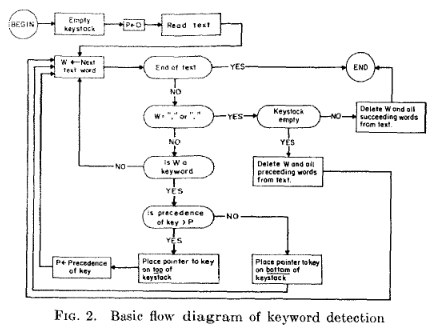
\includegraphics[width=1\textwidth]{eliza-keyword-detection.png}
    \caption{Flowchart de la détection des mots-clés (de l'article original sur ELIZA).}
    \label{fig:eliza-flowchart}
  \end{figure}

  \subsubsection{Substitution}
  On remarque aussi que dans l'exemple au-dessus, on a substitué le mot "you" à l'entrée par "I"
  à la sortie. De telles substitutions sont aussi définies dans la liste d'un mot-clé donné.  
  \todo[inline]{exemple.}
  
  \subsubsection{Classement des mots-clés}
  ELIZA contient aussi un mécanisme pour classer les mots clé par importance. D'où le besoin 
  pour ceci ? \todo[inline]{exemple.} Pendant le scan de la phrase à l'entrée, 
  ELIZA utilise une autre liste pour tenir compte des mots clé rencontrés, et pour les garder 
  ordonnés par leur importance.
  
  \subsubsection{Dernière réassemblage utilisé}
  Lorsqu'une règle de réassemblage correspondante à une décomposition 
  est utilisée, son indice est sauvegardé. 
  Lors de la prochaine utilisation de cette décomposition, cet indice 
  va permettre à ELIZA d'utiliser la règle de réassemblage qui suit la dernière utilisée. 
  Elle va utiliser chaque réassemblage avant de revenir sur un qu'on a déjà vu. 
  Ceci rend les réponses de ELIZA plus riches.
  
  \subsubsection{Mémoire}
  Un mécanisme très simple, mais qui pourtant produit des résultats impressionnants est celui 
  de la mémoire. Il permet à ELIZA de répondre à l'utilisateur même si aucun mot-clé n'est trouvé 
  dans l'entrée. La réponse va donc faire référence à quelque chose que l'utilisateur a dit 
  précédemment. Considérons la structure suivante : 

  \begin{center}
    (MEMORY MY \\
    (0 YOUR 0 = LETS DISCUSS FURTHER WHY YOUR 3) \\
    (0 YOUR 0 = EARLIER YOU SAID YOUR 3) \\
    ...)
  \end{center}

  Le mot-clé "MY" va alors servir à insérer des phrases dans la mémoire. Lorsque ce mot-clé 
  est choisi comme le plus important par le mécanisme de classement à la fin de la lecture 
  de l'entrée, l'une des transformations de la structure de mémoire est choisie aléatoirement. 
  Une copie de l'entrée est alors transformée est sauvegardée dans une pile. Le reste du processus 
  continue comme on l'a déjà décrit. Si jamais une entrée future n'admet aucun mot-clé, une réponse 
  est dépilée de la pile de mémoire et elle est envoyée à l'utilisateur. Ce mécanisme ajoute 
  beaucoup à l'effet que ELIZA pouvait produire sur ses utilisateurs. 

  \begin{figure}[h]
    \centering
    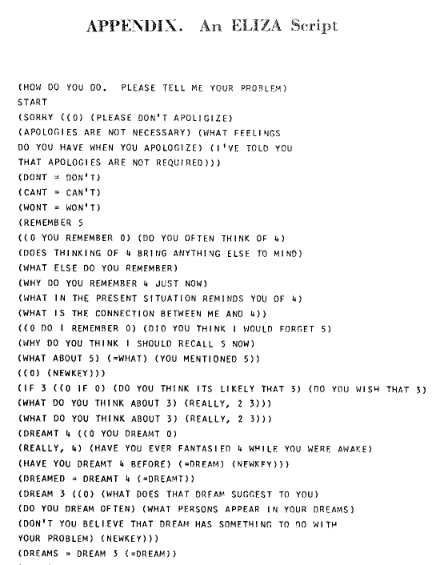
\includegraphics[width=0.8\textwidth]{eliza-script-example.png}
    \caption{Un script pour ELIZA (de l'article original sur ELIZA).}
    \label{fig:eliza-script}
  \end{figure}

      \subsubsection{Discussion}
Dans son livre \textit{Computer Power and Human Reason: From Judgement to Calculation}, 
Weizenbaum nous raconte des anecdotes parlant des premiers utilisateurs de ELIZA, 
qui devenaient parfois attachés émotionnellement au programme. Ou l'exemple de sa 
secrétaire, qui a apparemment demandé à Weizenbaum de sortir de la pièce pour qu'elle 
puisse avoir une vraie conversation avec ELIZA.  

\begin{quote}
  I had not realized that extremely short exposures to a relatively simple computer program could 
  induce powerful delusional thinking in quite normal people.
  \cite{weizenbaum-book}
\end{quote}

On pourrait alors considérer ELIZA comme l'un des premiers programmes capables de tenter 
le test de Turing, et aussi capable de le passer sous certaines conditions. 
D'après une étude réalisée à UC San Diego \cite{eliza-gpt} qui demandait à ses volontaires de converser 
par message soit avec un programme, soit avec un vrai humain, et de décider si la personne 
avec laquelle ils parlaient était un humain ou pas, ELIZA était plus performante que GPT 3.5. 
Ceci est assez incroyable, considérant la simplicité et légèreté d'ELIZA d'un point de vue 
informatique. Weizenbaum a réussi à créer un programme qui ne sait rien sur le monde réel, 
et qui arrive quand-même à tenir une conversation avec un humain en restant relativement 
convaincant. Tout ça en 1966 ! 

\begin{figure}[h]
  \centering
  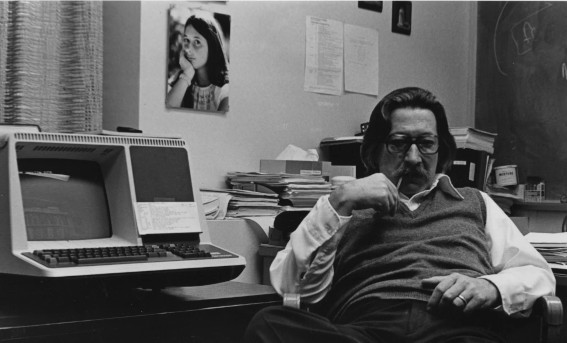
\includegraphics[width=0.8\textwidth]{weizenbaum.jpg}
  \caption{Joseph Weizenbaum en 1977.}
  \label{fig:weizenbaum}
\end{figure}

\textit{Il était intéressant de comparer ELIZA au programme de l'expérience de Georgetown-IBM. 
On voit que seulement en 12 ans, la complexité et les capacités des programmes ont augmenté 
énormément. Je m'en suis rendu compte aussi en écrivant ce rapport. Il m'a suffit de comparer 
le temps que j'ai mis à expliquer le fonctionnement du programme Georgetown-IBM, avec le temps 
que j'en ai mis pour ELIZA. Je trouve cette comparaison juste, car je crois que le niveau de 
détail que j'ai atteint dans les deux cas est à peu près le même. }


  \subsection{ALPAC report} 
  \cite{alpac-original}
  \cite{alpac-hutchins}
  ALPAC (Automatic Language Processing Advisory Committee) était une commission de 7 scientifiques, 
  dont le dirigeant John R. Pierce (un ingénieur américain), 2 linguistes, 2 chercheurs en traduction 
  automatique (TA en abrégé), un psychologue et un chercheur en IA, 
  crée par le gouvernement américain en 1964. Son but était d'évaluer le progrès de la 
  recherche en linguistique informatique, plus spécifiquement en traduction automatique. Son rapport 
  publié en 1966 est devenu célèbre pour sa critique de la TA comme domaine de recherche, 
  ainsi que pour l'explicitation du manque de résultats utiles après une dizaine d'années de recherche. 

  Le rapport se concentre sur les applications pratique de la TA, et comme on se trouve aux 
  États-Unis en 1966, ces applications consistent exclusivement à traduire des textes 
  (surtout scientifiques) du russe vers l'anglais. Le rapport répète que l'utilisation des 
  systèmes de TA tels qu'ils sont actuellement n'est pas envisageable. Les textes traduits 
  automatiquement ne sont pas très compréhensibles, ils ont donc besoin d'être revus et 
  corrigés par un humain. Ceci contredit la prémisse de la traduction automatique, qui justement est
  censée être \textit{automatique}. D'après le rapport, il serait plus économique et efficace 
  de garder la tâche de traduction chez les traducteurs humains, et de rediriger les financements 
  ailleurs. 

  \begin{figure}[t]
    \centering
    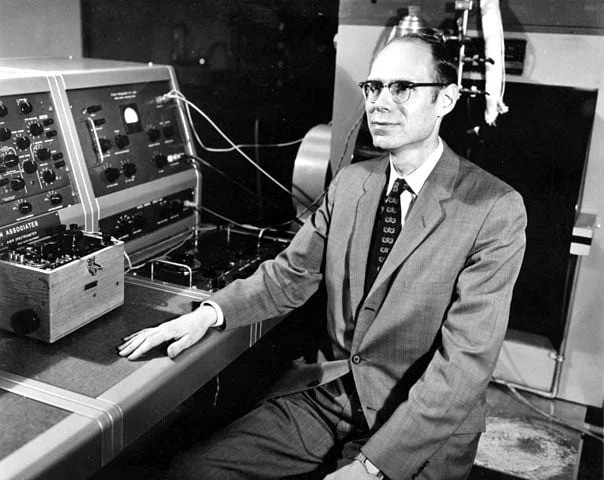
\includegraphics[width=0.6\textwidth]{pierce.jpg}
    \caption{John R. Pierce (dirigeant de la commission ALPAC).}
    \label{fig:pierce}
  \end{figure}

  Les effets de ce rapport ont été sévère pour le domaine, même s'il y a des parties du rapport qui sont 
  contestables. On peut aussi remarquer qu'il essaye d'accentuer "l'échec" de la TA. 
  Par exemple, le rapport fait une comparaison entre le programme de l'expérience Georgetown-IBM 
  (dont on a déjà parlé) et les systèmes de TA actuels (10 ans plus tard), en essayant de montrer que les résultats 
  de ce premier étaient plus impressionnants. Je pense que nous allons tous être 
  d'accord qu'une telle comparaison est ridicule. Comparer un "programme-dictionnaire" capable 
  de traduire 60 phrases spécifiquement choisies, avec des modèles qui traduisent des textes 
  quelconques (même si pas parfaitement) n'est pas très correcte. Le rapport gonfle aussi les 
  financements qui ont été attribués aux recherches en TA. 20 millions de dollars d'après le rapport, mais en réalité 
  il s'agissait plutôt de 12 ou 13 millions de dollars. 
  
  On peut dire que le rapport n'a vu la traduction automatique que comme un outil des 
  motivations stratégiques et politiques de l'époque, qui était 
  déjà censé fonctionner, et qui n'en était pas capable. Il est vrai que les résultats 
  de la TA étaient parfois décevants, et qu'une application dans la vraie vie n'était pas encore possible. 
  Malheureusement, le rapport n'a pas reconnu le potentiel de la TA, et sa publication 
  a beaucoup endommagé le développement du domaine.   

  \section{Approche statistique}
  \subsection{Note historique}
  Jusqu'aux années 1980s, l'approche symbolique dominait le traitement automatique du langage, 
  c'est-à-dire des systèmes utilisant un grand nombre de règles écrites à la main. Listons deux
  choses (parmi plusieurs évidemment) qui ont motivé le changement qui est apparu dans les années 
  1980s. 

  Premièrement, les théories linguistiques dites \textit{Chomskyennes} perdaient en popularité
  (après le linguiste américain Noam Chomsky). Ces théories couvrent évidemment un grand nombre 
  de sujets linguistiques différents. Pour simplifier énormément, on peut dire que ces théories 
  présentent d'une façon ou d'une autre le point de vue, que tout langage peut être décrit par 
  un ensemble de règles. Ce n'est pas par hasard si ça nous rappelle l'approche symbolique. 
  Par exemple, dans son livre \textit{Syntactic Structures} de 1957, Noam Chomsky argumente 
  que le langage n'est pas une habitude ou une capacité que l'humain apprend pendant sa vie, 
  mais que cette capacité est codée dans nos cerveaux, comme quelque chose de purement génétique.
  Ces deux opinions différentes sur l'origine du langage se traduisent très facilement sur l'histoire 
  du TALN. L'opinion de Noam Chomsky représente l'approche symbolique, qui essaie de trouver une 
  explication globale pour le problème avec un ensemble de règles. L'opinion dite "béhavioriste" : 
  le langage étant une capacité qui s'apprend pendant la vie, représente l'approche statistique 
  et surtout neuronale. Un algorithme d'apprentissage automatique qui apprend des données 
  numérique comme un humain apprend de ces expériences. En regardant l'état actuel du domaine, 
  on dirait que Chomsky avec tort. 
  
  Un autre facteur était l'augmentation de la puissance des ordinateurs. Ceci a permis l'utilisation 
  des algorithmes d'apprentissage automatique et l'entraînement des modèles toujours plus grands. 

  \subsection{N-grammes}
  \cite{stanford-book-ngrams}
  \subsubsection{Introduction}
  L'idée à la base des n-grammes est la suivante : étant donné le début d'une phrase, peut-on 
  deviner le mot qui suivra ? Cette idée est assez naturelle et intuitive. Essayons de poser 
  une question plus mathématique. Par exemple : étant donné le début d'une phrase, quelle est la \textbf{probabilité}
  qu'un mot spécifique suivra ? Les modèles qui répondent à cette question s'appellent des 
  \textit{modèles de langage} (\textit{language models} en anglais). Même si ce nom semble 
  très général, il n'est donné qu'aux modèles qui cherchent la probabilité qu'un mot spécifique 
  suivra, et les n-grammes en font partie. Les modèles actuels comme GPT sont des \textit{large language models}. Eux aussi essaient 
  de deviner le mot qui suivra, mais à grâce à leurs proportions énormes, on ajoute le mot 
  \textit{large} pour les nommer. On peut aussi attribuer une probabilité à une phrase 
  entière. Laquelle des deux phrases suivante a une plus grande probabilité d'apparaître 
  dans un vrai texte ? 
  \begin{align*}
    &\textup{J'ai passé le matin à travailler sur le rapport qu'on doit rendre ce vendredi.} \\
    &\textup{Travailler à vendredi le rendre passé sur le j'ai matin qu'on ce doit rapport.}
  \end{align*}
  
  \subsubsection{Cas d'usage}
  Ces probabilités nous permettent de choisir la meilleure option : plus probable $\approx$ plus 
  correcte. Ceci est utilisé fortement dans l'autocomplétion et dans l'autocorrection. 

  Le cas d'usage pour l'autocomplétion est évident. Une fois qu'on a frappé \textit{Je pense}, 
  le système propose les mots qui sont les plus probable à suivre ce début de phrase : 
  \textit{que}, \textit{qu'il}, \textit{qu'on}. En plus, on peut utiliser l'historique du 
  texte qu'on a écrit pour mettre à jour le corpus sur lequel le modèle calcule les 
  probabilités. On peut ainsi adapter et améliorer en continu le système.  
  
  Avec un modèle 
  de langage, on peut se rendre compte que la probabilité que les mots \textit{à chaque foi\underline{d}}
  apparaissent dans un texte est quasiment 0, même si la probabilité que les mots \textit{à chaque} 
  apparaissent ensemble est assez grande. Le problème se trouve alors dans les deux derniers mots. 
  Le modèle peut nous dire que la probabilité des mots \textit{chaque fois} est beaucoup plus grande 
  que celle de \textit{chaque foi\underline{d}}, et on corrige ainsi une erreur de frappe. 

  Ou bien imaginons qu'on veut écrire 
  la phrase \textit{Ils sont contents.}, mais grâce à une faute de frappe, on finit avec 
  \textit{Ils ont contents.} Cette phrase est "correcte" dans le sens que chacun de ses mots 
  est bien un mot français, ce qui n'était pas le cas dans l'exemple précédent.
  Ceci rend la faute plus difficile à trouver. Pourtant, avec un modèle de langage, 
  on peut voir que la probabilité qu'un adjectif (\textit{contents}) suive 
  les mots \textit{ils ont} est quasiment 0. 
  \begin{quote}
    Exercice pour le lecteur : trouver une phrase 
    française grammatiquement ET sémantiquement correcte où \textit{ils ont} est suivi d'un 
    adjectif. Tout ce que j'ai trouvé, ce sont des phrases où ce n'est pas le cas. 
    \begin{align*}
      &\textup{Ils ont \underline{trois} chiens. (un numéral)}\\
      &\textup{Ils ont \underline{une} voiture. (un article)}\\
      &\textup{Ils ont \underline{peur}. (un nom)}
    \end{align*}
  \end{quote} 
  Ceci nous dirait qu'il y ait très probablement un truc qui ne va pas dans cette phrase. 
  On peut alors avertir l'auteur et corriger une faute qu'on n'aurait pas vu sinon. 

  On peut aussi corriger des erreurs grammaticales. La probabilité que le mot 
  \textit{passé} suive les mots \textit{j'ai} et beaucoup plus grande que 
  pour le mot \textit{passer}, ce qui nous permet de corriger une erreur de conjugaison. 
  

  Un autre cas d'utilisation est dans la récognition de voix. Les deux séquences de mots
  suivante se prononce de la même façon, mais il est clair que c'est la première qu'on veut 
  reconnaître, plutôt que la deuxième. 
  \begin{align*}
    &\textup{... ma chère mère danse ...}\\
    &\textup{... ma chaire mer dent ce}...\\
  \end{align*}
  En déterminant que la première phrase a une probabilité beaucoup plus grande d'exister 
  dans un texte que la deuxième (ce qui nous dira notre modèle de langage), 
  le système peut faire le bon choix. 

  Finalement, les modèles de langage sont utiles dans la CAA (communication améliorée et 
  alternative). Les personnes qui ne sont pas capables de parler ni d'utiliser la langue des 
  signes utilisent parfois leur vue ou d'autres mouvement spécifiques pour choisir des mots 
  d'une sélection. Un modèles de langage peut alors fournir des meilleures prédictions et 
  faciliter la communication. 

  \subsubsection{Principe}
  Voici la façon naïve de faire. On essaie de trouver $P(w|h)$ : la probabilité que le mot 
  $w$ suive l'historique $h$ (le début d'une phrase par exemple). Prenons $w = \textup{que}$ et 
  $h = \textup{c'est sûr}$. On pourrait calculer cette probabilité ainsi : 
  \begin{align}
    P(w|h) = \frac{C(\textup{c'est sûr que})}{C(\textup{c'est sûr})}
  \end{align}
  où $C(\textup{c'est sûr que})$ est le nombre de fois que "c'est sûr que" apparaît 
  dans le corpus, et $C(\textup{c'est sûr})$ est défini analogiquement. Cette approche 
  ne marchera pas à cause de la variabilité du langage. Le nombre de séquences de mots
  ou de phrases  
  correctes est tout simplement trop grand, même pour un corpus énorme comme le web.
  Ceci veut dire qu'on ne saurait pas compter le nombre de fois qu'une séquence apparaît
  dans le corpus, car elle y serait pas, même si elle serait tout à fait plausible et 
  correcte. 

  Voilà où entrent en scène les n-grammes. Par exemple avec un \textit{bigramme}, 
  au lieu de trouver la probabilité en comptant les occurrences de 
  "c'est sûr" et de "c'est sûr que", on va l'approximer en calculant la probabilité que "que" suive 
  le dernier mot de l'historique : "sûr". Pour un \textit{trigramme}, ça serait 
  la probabilité que "que" suive les 2 derniers mots de l'historique : \textit{c'est sûr}.
  
  En gros, un n-gramme va approximer la probabilité qu'un mot $w_k$ suive une séquence 
  de mots $w_{1}, w_{2} \dots w_{k-1}$ en seulement considérant les n-1 derniers mots. 
  En calculant une probabilité conditionnelle sur ces n-1 derniers. 
  De gauche à droite : la probabilité qui nous intéresse, son approximation par un bigramme, 
  et son approximation par un trigramme. 
  \begin{align}
    P(w_n|w_1, w_2, \dots w_{n-1}) \approx P(w_n|w_{n-1}) \approx P(w_n|w_{n-2}, w_{n-1})
  \end{align}

  La supposition ou la propriété qu'on peut deviner le prochain mot juste en regardant quelques mots en arrière 
  qui est faite par les n-grammes, s'appelle la \textit{propriété de Markov}. Celle-ci parle 
  d'une absence de mémoire d'un système : l'état futur ne dépend que de l'état présent, et 
  non pas des états passés. 

  \subsubsection{En pratique}
  Imaginons qu'on ait un corpus de texte donné, sur lequel on veut calculer les bigramme 
  probabilités. On construit une matrice où les lignes et les colonnes sont indexées par 
  les mots du corpus. La case sur la ligne \textit{sûr} et la colonne \textit{que} contient 
  le nombre de fois que \textit{sûr que} apparaît dans le corpus. Pour convertir cela 
  en probabilités, il suffit de normaliser cette case par le nombre d'occurrences de \textit{sûr}
  dans le corpus. La probabilité de la phrase \textit{C'est sûr que oui.} serait alors 
  calculée ainsi : 
  \begin{align*}
    P(\textup{C'est sûr que oui.}) = P(\textup{c'est}|<)
    P(\textup{sûr}|\textup{c'est})P(\textup{que}|\textup{sûr})
    P(\textup{oui}|\textup{que})P(>|\textup{oui})
  \end{align*}
  où $<$ et $>$ sont des symboles représentant le début et la fin d'une phrase du corpus.
  C'est une extension purement technique qui nous permet d'exprimer la probabilité 
  conditionnelle des mots qui se trouvent au début ou à la fin d'une phrase, en traitant 
  ces symboles comme des mots du corpus. 

  Une telle matrice va contenir beaucoup de cases de valeur 0. Celles-ci correspondent à 
  des binômes de mots qui ne se trouvent pas dans notre corpus. Pourtant, un tel binôme 
  peut très bien apparaître dans la "vraie vie", et notre modèle lui associerait une 
  probabilité 0, ce qui n'est évidemment pas correct. Pour remédier à ceci, il existe 
  plusieurs techniques de \textit{lissage}, qui redistribuent les probabilités du modèle, 
  à ce que les cases qui avaient initialement une probabilité 0 aient une probabilité
  positive. 

  En pratique, les probabilités des modèles de langage sont toujours exprimées dans 
  l'espace logarithmique. Au lieu de travailler avec  
  \begin{align}
    P = p_1 p_2 p_3
  \end{align}
  on travaille avec 
  \begin{align}
    P = \textup{exp}(\textup{ln} \ p_1 + \textup{ln} \ p_2 + \textup{ln} \ p_3)
  \end{align}
  La raison pour ceci est que les probabilités sont par définition des flottants entre 
  0 et 1. En multipliant plusieurs probabilités, on peut donc facilement arriver à ce qu'on 
  appelle un \textit{soupassement arithmétique} (\textit{arithmetic underflow}) : une 
  valeur qui est trop précise pour être calculée par l'ordinateur. Elle serait alors 
  traîtée comme 0, ce qui n'est pas ce qu'on cherche. L'espace logarithmique nous permet 
  d'échapper à ce problème, en transformant la multiplication en addition. 

  \begin{figure}[t]
    \centering
    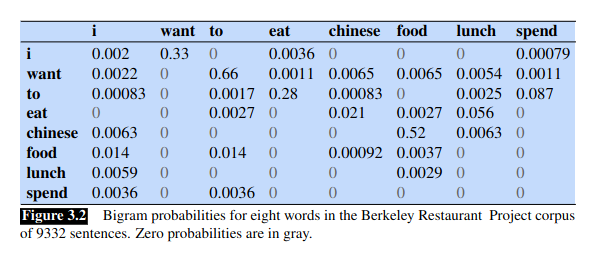
\includegraphics[width=1\textwidth]{bigram.png}
    \caption{Exemple de bigramme probabilités \cite[\textit{Speech and Language Processing}]{stanford-book-ngrams}.}
    \label{fig:pierce}
  \end{figure}

  Il est essentiel de bien choisir les jeux d'entraînement, de validation et de test. 
  Le jeu d'entraînement représente le corpus de texte sur lequel on calcule les 
  probabilités. Le jeu de validation sert à tester le modèle pendant son développement. 
  Le jeu de test sert à évaluer le modèle final. Il est important que les jeux 
  d'entraînement et de test soient disjoints, pour ne pas produire des résultats biaisés. 

\chapter{Word embedding}
  \section{Introduction}
  \cite{wikipedia-wembedding} \cite{wikipedia-wembedding-fr} Le word embedding (en français : vectorisation de mots, plongement lexical, ou bien enchâssement de mots)
est la notion de représenter un mot par un vecteur (réel), en sorte que ça code leur sémantique.
L'idée principale étant que dès qu'on a des vecteurs, on peut faire des maths dessus. Et si ce 
codage de nos mots est bien fait, on s'attend à ce que les opérations mathématiques qu'on peut 
faire sur les vecteurs correspondent à des relations sémantiques entre nos mots. 

Par exemple, on pourrait se demander quel est le vecteur le plus proche du vecteur qui représente 
le mot "chien". Si notre word embedding est bien fait, on s'attend à trouver dans sa proximité 
les vecteurs des mots comme "chiot", "Rex", "berger", etc. 

On peut aussi additionner des vecteurs. Imaginons qu'on prend le vecteur du mot "repas", et on lui 
ajoute le vecteur du mot "viande". On voudrait que le vecteur résultat soit proche des vecteurs 
des mots comme "steak haché", "poulet rôti", "boef bourgignon", "guláš", etc. 

La soustraction nous donne l'exemple le plus connu du word embedding, qui mathématiquement 
s'exprime ainsi : 
\begin{align*}
  \overrightarrow{roi} \ - \ \overrightarrow{homme} \ + \ \overrightarrow{femme} \approx \overrightarrow{reine}
\end{align*}

Comme le dernier exemple : ça serait quoi la moyenne entre les vecteurs des mots "nuit" et "jour" ?


Grâce à cette représentation numérique, on obtient des nombreuses 
possibilités d'analyse sémantique de texte. On peut trouver les mots les plus similaires à un mot donné, 
et on peut faire pareil pour les phrases (moteurs de recherche, autocorrection). Pour obtenir 
le vecteur d'une phrase, il suffit de prendre la moyenne des vecteurs de ses mots.  
On peut analyser de différents documents et obtenir un résumé de leur contenu, de l'opinion 
ou de l'émotion qui se trouve dedans. On peut mesurer la similarité entre documents, sémantiquement
parlant. 

Les word embedding sont également essentiels pour l'apprentissage automatique. 
Ici, ils servent d'un prétraitement avant de passer les données au modèle de ML ou de DL. 
On a bien besoin de représenter nos données textuelles par quelque chose mathématique (des vecteurs), 
si on veut les passer à un modèle d'apprentissage automatique. Ainsi le nombre de cas d'usage 
du word embedding devient énorme. 

\begin{figure}[h]
  \centering
  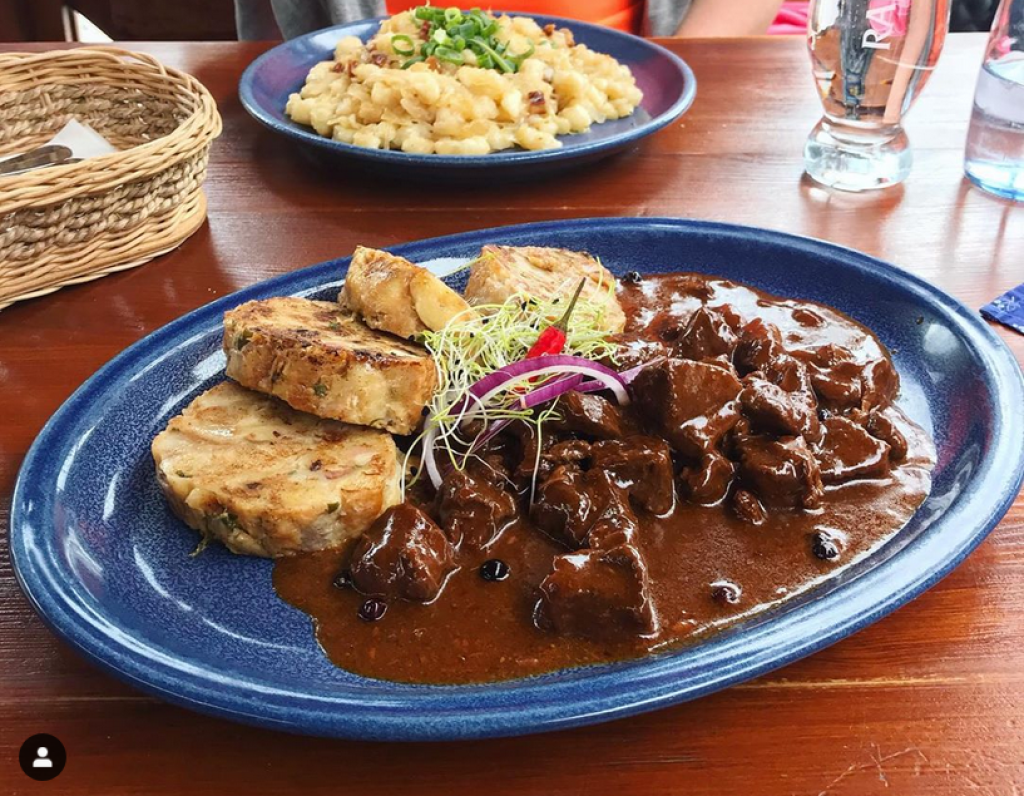
\includegraphics[width=0.6\textwidth]{gulas.png}
  \caption{Guláš.}
  \label{fig:gulas}
\end{figure}


  \section{Principe sur un exemple simple}

  \begin{figure}[h]
    \centering
    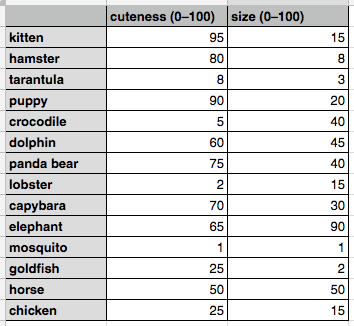
\includegraphics[width=0.6\textwidth]{animal-table.png}
    \caption{Word embedding d'animaux.}
    \label{fig:animaux-word-embedding}
  \end{figure}

Regardons maintenant un word embedding concret, très simple. Ce qui suit dans cette 
section est essentiellement une 
traduction de \cite[\textit{Understanding word vectors}, Allison PARISH]{understanding-word-vectors} 
en français. Considérons la table dans fig. \ref{fig:animaux-word-embedding} qui décrit quelques 
animaux en fonction de leur mignonnerie et leur taille. 

Sur fig. \ref{fig:animaux-word-embedding-2d}, vous pouvez voir 
ce que ça donne en tant qu'espace de vecteurs 2D. 
Cet exemple très simple est bien un word embedding : on a associé un vecteur 2d à chaque mot 
de notre table. Certes, d'une façon arbitraire, mais pourtant intuitive, et on croit que les 
valeurs qu'on a choisies codent bien les relations sémantiques entre nos animaux. On peut désormais 
tester les opérations dont on a parlé dans la partie précédente, pour voir si notre word embedding 
est bien fait. 
\begin{figure}[!htb]
  \centering
  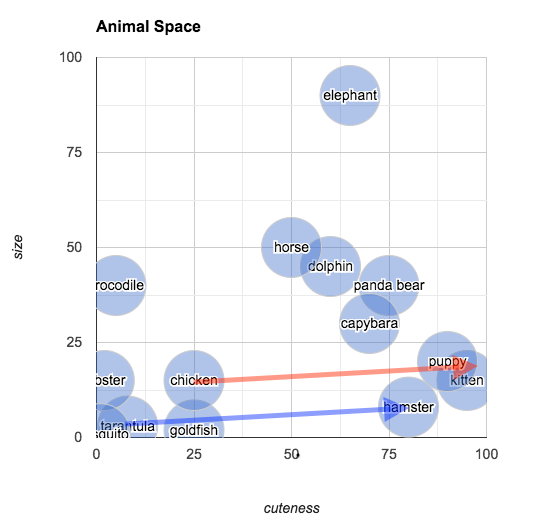
\includegraphics[width=0.6\textwidth]{animal-space-dif.png}
  \caption{La tarentule au hamster.}
  \label{fig:tarentule-hamster}
\end{figure}

Remarquons que le cheval et le dauphin sont proches l'un de l'autre. Deux animaux assez mignons et grands, 
d'après notre embedding (même si les dauphins ne sont parfois pas si mignons que ça...). Similairement pour 
le chaton et le chiot, deux animaux qui sont petits et très mignons, ou bien la tarentule et le moustique, 
très petits et pas du tout mignons. Prenons maintenant la différence entre le chaton et le poussin et ajoutons-la 
à la tarentule. Voyons ceci sur la fig. \ref{fig:tarentule-hamster}. 

La pointe du vecteur bleu est le plus près du vecteur qui représente le hamster.
Mathématiquement, cela s'écrirait :
\begin{align*}
  \vec{c} - \vec{p} + \vec{t} \approx \vec{h} 
\end{align*}
Et en français : 
\begin{center}
  Les tarentules sont aux hamsters ce que les poussins sont aux chatons. 
\end{center}
C'est-à-dire un animal un peu plus petit et beaucoup moins mignon, ce qui est assez 
correcte. On suppose ici que les poussins sont moins mignons que les chatons... bon, 
il y a pas mal de gens qui seraient d'accord, on le laisse comme ça. 

On a vu un word embedding sur quelques mots d'animaux, qui nous a permis d'analyser leur sémantique.  
On associe un vecteur à chaque mot en fonction de la mignonnerie et la 
taille de l'animal, on regarde la relation mathématique entre deux mots
(le poussin et le chaton), et on utilise cette information pour déduire une \textbf{relation sémantique} 
entre deux mots différents (la tarentule et le hamster). 
Incroyablement simple et puissant en même temps.


\section{Sémantique distributionnelle}
\begin{quote}
  You shall know a word by the company it keeps. \newline
  J. R. Firth, 1957
\end{quote}
\cite{wikipedia-distributional-semantics} 
\cite{firth-pic}
Dans les applications réelles des word embeddings, le principe reste le même, mais le processus devient plus 
compliqué. Les mots à l'entrée vont être beaucoup plus nombreux - on peut imaginer un ensemble 
des centaines de milliers de mots. Ensuite, comment fait-on pour associer un vecteur à chacun
de ces mots ? Dans l'exemple précédent, on a attribué des valeur arbitraires à chaque mot 
manuellement, ce qui ne sera plus possible à cause de leur quantité. On veut aussi quelque chose de général et 
automatisable. On veut qu'un ordinateur soit capable de produire le word embedding, sans devoir philosopher 
sur la question : est-ce qu'un poussin est plus mignon qu'un chaton ? Heureusement qu'il y a la 
hypothèse distributionnelle. 

\begin{hyp}[hypothèse distributionnelle]
  La sémantique d'un mot est déterminée par son contexte - les mots qui l'entourent dans 
  le texte. 
\end{hyp}

Cette hypothèse dûe à J. R. Firth (linguiste britannique des années 1950s) nous dit que ce qui détermine la 
sémantique d'un mot, ce sont les mots qui se trouvent à ses côtés dans la phrase. Prenons les mots 
\textit{beau}, \textit{froid} et \textit{chaud}, et regardons des exemples de 
phrases qui les emploient : 

\begin{center}
  Il a fait \underline{bien} \textbf{froid} \underline{hier}. \\
  Par contre, il va faire \underline{hyper} \textbf{chaud} \underline{aujourd'hui}. \\
  Il fera \underline{très} \textbf{beau} \underline{demain}! \\
  Est-ce qu'il va faire \underline{très} \textbf{froid} \underline{mardi} ?
\end{center}

Il s'agit des phrases naturelles, et on peut déjà observer que les trois mots 
ont une tendance à se trouver entre un adverbe (bien, hyper, très) et un mot indiquant 
un jour (hier, aujourd'hui, demain, mardi). Par la hypothèse distributionnelle, ces trois mots 
devraient avoir une sémantique similaire, car ils ont le même 
contexte. Ceci est tout à fait vrai, tous les trois mots sont utilisés pour décrire le temps. 
Une telle sémantique s'appelle alors comme la hypothèse - distributionnelle. 

Cette approche nous permettra d'associer des vecteurs aux mots d'une entrée de taille 
arbitraire, et en plus automatiquement. Regardons sur un exemple provenant de \cite{understanding-word-vectors} :
\begin{center}
  It was the best of times, it was the worst of times.                                                                                                                                                                                                                                                                                                                                                                                                                                                                                                                                                                                                                                                                                                                                                                                                                                                                                                                                                                                                                                                                                                                                                                                                                                                                                                                                                                                                                                                                                                                                                                                                                                                                                                                                                                                                                                                                                                                                                                                                                                                                                                                                                                                                                                                                                                                                                                                                                                                                                                                                                                                                                                                                                                                                                                                                                                                                                                                                                                                                                                                                                                                                                                                                                                                                                                                                                                                                                                                                                                                                                                                                                                                                                                                                                                                                                                                                                                                                                                                                                                                                                                                                                                                                                                                                                                                                                                                                                                                                                                                                                                                                                                                                                                                                                                                                                                                                                                                                                                                                                                                                                                                                                                                                                                                                                                                                                                                                                                                                                                                                                                                                                                                                                                                                                                                                                                                                                                                                                                                                                                                                                                                                                                                                                                                                                                                                                                                                                                                                                                                                                                                                                                                                                                                                                                                                                                                                                                                                                                                                                                                                                                                                                                                                                                                                                                                                                                                                                                                                                                                                                                                                                                                                                                                                                                                                                                                                                                                                                                                                                                                                                                                                                                                                                                                                                                                                                                                                                                                                                                                                                                                                
\end{center}
Comme le contexte, on considérera juste le voisin de gauche et le voisin de droite de chaque mot. La 
première ligne de la table \ref{tab:sémantique-distr-exemple} contient tous les contextes possibles 
Même si "it was the" a deux occurrences dans notre phrase, le contexte correspondant 
"it \textunderscore \ the" ne se trouve qu'une fois dans la table. On prend les contextes sans répétition.
La première colonne contient tous les mots, aussi sans répétition.
Finalement, pour chaque mot, les valeur dans sa ligne indique combien de fois il se trouve dans le contexte
spécifié.  

\begin{table}[h]
    \resizebox{1.2\textwidth}{!}{%
    \begin{tabular}{|c|*{10}{c|}}
        \hline
        g & 
        DÉBUT \textunderscore \ was & 
        it \textunderscore \ the & 
        was \textunderscore \ best & 
        the \textunderscore \ of & 
        best \textunderscore \ times & 
        of \textunderscore \ it & 
        times \textunderscore \ was & 
        was \textunderscore \ worst & 
        worst \textunderscore \ times & 
        of \textunderscore \ FIN \\
        \hline
        it & 1 & 0 & 0 & 0 & 0 & 0 & 1 & 0 & 0 & 0 \\ 
        \hline
        was & 0 & 2 & 0 & 0 & 0 & 0 & 0 & 0 & 0 & 0 \\
        \hline
        the & 0 & 0 & 1 & 0 & 0 & 0 & 0 & 1 & 0 & 0 \\
        \hline 
        best & 0 & 0 & 0 & 1 & 0 & 0 & 0 & 0 & 0 & 0 \\
        \hline 
        of & 0 & 0 & 0 & 0 & 1 & 0 & 0 & 0 & 1 & 0 \\
        \hline 
        times & 0 & 0 & 0 & 1 & 0 & 0 & 0 & 0 & 0 & 1 \\
        \hline 
        worst & 0 & 0 & 0 & 1 & 0 & 0 & 0 & 0 & 0 & 0 \\
        \hline  
    \end{tabular}%
    }
    \caption{Contextes d'une phrase.} 
    \label{tab:sémantique-distr-exemple} 
\end{table}

\begin{figure}[h]
  \centering
  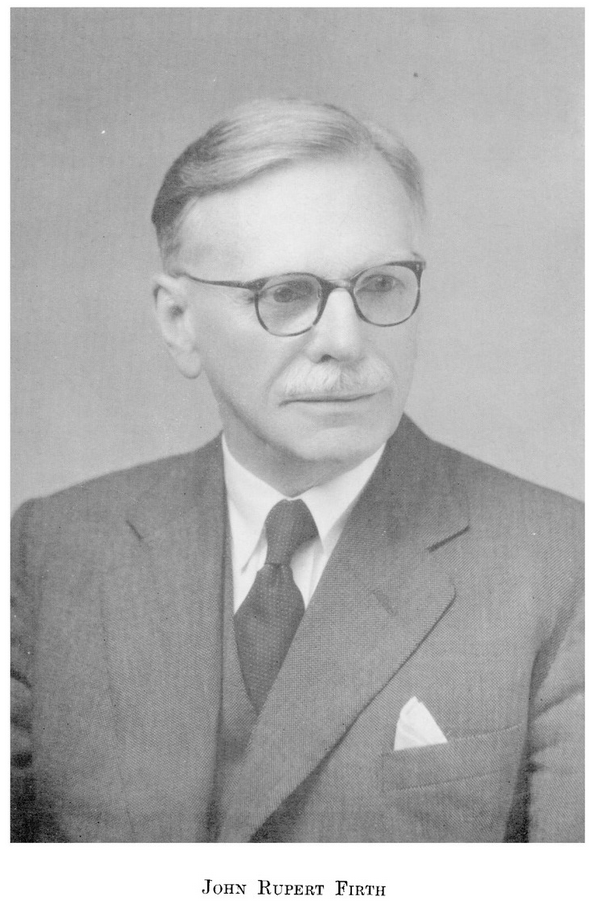
\includegraphics[width=0.3\textwidth]{firth.png}
  \label{fig:firth}
\end{figure}

On observe que les vecteurs des mots \textit{best} et \textit{worst} sont les mêmes :
$[0,0,0,1,0,0,0,0,0,0]$. La distance euclidienne entre les deux est zéro, et par la 
hypothèse distributionnelle, ces deux mots devraient avoir la même signification. Ce n'est pas 
tout à fait le cas, car \textit{best} et \textit{worst} sont des antonymes, pas des synonymes. 
Pourtant, leurs sémantiques sont très proches, et on a réussi à le reconnaître.
Cette façon d'obtenir un word embedding s'appelle \textit{count-based} : on compte le nombre de fois 
qu'un mot apparaît dans un contexte pour obtenir son vecteur.  

Dans l'exemple précédent, notre corpus (l'entrée textuelle) consistait en une phrase, ce qui 
nous a donné 10 contextes : 10 positions possibles pour un mot.  
En réalité, on est amené à utiliser des corpus beaucoup plus grands, où on aurait donc des 
milliers ou mêmes des millions de contextes possibles - des vecteurs à des milliers ou des 
millions de dimensions. On se doute que ce ne serait pas très 
pratique. Grâce à des techniques de réduction de dimensionnalité, on peut transformer des vecteurs 
énormes en vecteurs de dimension plus raisonnable : environ 100-300, sans perdre trop 
d'information. Je laisse les détails de cette 
transformation de côté (c'est des maths).

\section{Démonstration}
Il existe de nombreuses collections de vecteurs déjà prêtes qu'on 
peut télécharger et utiliser dans nos projets. Dans l'exemple suivant, 
on utilisera la collection \textit{en\_core\_web\_lg}, disponible dans la bibliothèque Python 
\textit{SpaCy}. Il s'agit de 514 000 vecteurs de mots 
anglais à 300 dimensions, provenant de plusieurs sources. 
Ça fait beaucoup de vecteurs. 

Cette démonstration est elle aussi fortement inspirée par
\cite[\textit{Understanding word vectors}, Allison PARISH]{understanding-word-vectors} (tout ce que j'ai changé c'est le livre),
comme je ne suis pas très original et surtout je n'ai pas le temps de développer un exemple intéressant 
moi-même. Pour cela, il faudrait vraiment plonger dans le sujet, et ce n'est pas 
possible, sachant qu'on est à la fin du semestre :)

Je vais utiliser l'un de mes livres préféré comme le corpus : 
\textit{Joyland}, écrit par Stephen King. Pour vous mettre un peu dans l'ambiance, 
\textit{Joyland} parle d'un jeune homme du nom Devin Jones. Devin a 21 ans, il fait 
des études d'anglais, il rêve de devenir écrivain, mais sinon il ne sait pas 
quoi faire de sa vie. Sa copine vient de le larguer, et donc au lieu de 
passer les vacances d'été avec elle, il les passe à travailler dans un parc 
d'attraction. Ici il trouve des amis et un boulot qui lui plaît. Un peu plus tard, 
il fait enfin la connaissance de la jolie femme blonde qui habite dans l'une des maisons 
qui bordent la plage que Devin traverse pour se rendre au parc. Il y a aussi 
un mystère à résoudre (c'est du Stephen King) : une suite de meurtres de jeunes 
filles, toutes dans des parcs d'attraction, incluant celui où Devin passe son été. 
Tout ça dans une vibe des années 70 en Caroline du Nord. 

On va charger le texte de \textit{Joyland} comme l'entrée, et on va utiliser les 
vecteurs déjà disponibles dans \textit{SpaCy} pour analyser ce texte. On va utiliser que 
des mots unique du livre, et en plus que des mots du livre qui ont un vecteur dans le 
modèle. Les relations sémantiques sont déterminées par le modèle déjà entraîné, mais 
les résultats vont quand même nous donner des informations sur notre entrée spécifique. 
Cet exemple représente ce qui se passe lorsqu'on utilise un word embedding pour analyser 
la sémantique d'un document, par exemple pour déterminer l'émotion principale d'un commentaire.
Voici le code (les commentaires sont en anglais mais je crois que ça ira) \cite{gensim-tuto}: 

\begin{lstlisting}[language=Python]
  from __future__ import unicode_literals
  import spacy 
  import numpy as np 

  # load the word vectors into our model 
  nlp = spacy.load("en_core_web_lg")
  # read the text (joyland.txt) and create our corpus (doc)
  doc = nlp(open("joyland.txt").read())

  # keep only alphabetical words and lowercase them 
  tokens = list(set([w.text.lower() for w in doc if w.is_alpha]))
  # keep only words that have a vector in our model 
  tokens = list(filter(lambda x: nlp.vocab.has_vector(x), tokens))
  # extract sentences
  sentences = list(doc.sents)

  """ Calculates the cosine similarity between two vectors. """
  def cos_sim(u, v):
    return np.dot(u, v)/np.linalg.norm(u)/np.linalg.norm(v)

  """ Returns the vector corresponding to the input string. """
  def vec(s : str):
    return np.array(nlp.vocab[s].vector)

  """ Return the word corresponding to the given vector by looking 
  for the closest vector in the model.
  """
  def word(v):
    max_sim = -1 
    res = ""
    for w in nlp.vocab:
      if w.has_vector:
        sim = cos_sim(v, w.vector)
        if sim > max_sim:
          max_sim = sim 
          res = w.text
    return res  

  """ Return the list of most similar words to the given one. """
  def closest_words(token_list, v, n=5):
    return sorted(token_list, 
                    key=lambda x: cos_sim(vec(x), v), 
                    reverse=True)[:n]

  """ Return closest sentences """
  def closest_sents(sents_list, sent, n=5):
    return sorted(sents_list, 
                  key=lambda x: cos_sim(x.vector, nlp(sent).vector), 
                  reverse=True)[:n]
\end{lstlisting}

Regardons quelques exemples de mots les plus similaires. Il y a des similarité 
purement grammaticales, mais aussi des similarités sémantiques très intéressantes.
\begin{lstlisting}[language=Python]
  >>> print(closest_words(tokens, vec("food")))
['food', 'seafood', 'meat', 'cooking', 'meal']
>>> print(closest_words(tokens, vec("love")))
['love', 'loves', 'loved', 'loving', 'lovers']
>>> print(closest_words(tokens, vec("friend")))
['friend', 'ladyfriend', 'girlfriend', 'friends', 'boyfriend']
>>> print(closest_words(tokens, vec("dog")))
['dog', 'dogs', 'cat', 'pet', 'pup']
>>> print(closest_words(tokens, vec("happy")))
['happy', 'unhappy', 'grateful', 'excited', 'happily']
\end{lstlisting}  

Un exemple classique consiste à trouver le mot à mi-chemin entre \textit{day} et 
\textit{night}.
\begin{lstlisting}[language=Python]
  >>> v = (vec("day") + vec("night"))/2
  >>> print(closest_words(tokens, v))
  ['day', 'night', 'morning', 'evening', 'afternoon']
\end{lstlisting}  

Ajoutons maintenant le vecteur de \textit{meat} à \textit{food}.
Toujours un bon dîner mais un peu plus carnivore. 
\begin{lstlisting}[language=Python]
  >>> print(closest_words(tokens, vec("food")))
  ['food', 'seafood', 'meat', 'cooking', 'meal']
  >>> print(closest_words(tokens, vec("food") + vec("meat")))
  ['food', 'meat', 'seafood', 'chicken', 'pork']
\end{lstlisting}  

\section{Word2Vec}
\subsection{Introduction}
\cite{wikipedia-word2vec} \cite{wikipedia-word2vec-fr} Word2Vec est utilisé comme le nom commun de deux architectures de réseau neuronale, créés par 
une équipe de chercheurs à Google en 2013. Leurs deux modèles : CBOW et Skip-gram, étaient plus 
rapide et plus précise que les autres modèles qui existaient à l'époque. Ils étaient capable 
de produire un word embedding sur un corpus de 1.6 milliards de mots en moins d'un jour \cite{word2vec-original}.
Ils ont marqué un énorme progrès dans le domaine. Par conséquence, les word embedding sont 
devenu beaucoup plus populaires et utilisés. Ces modèles sont \textit{prediction-based} : on 
entraîne les modèles à deviner soit le contexte étant donné un mot, soit le mot étant donné
son contexte. On verra dans la suite comment on obtient un vecteur à partir de cette prédiction.
Remarquons la différence avec les modèles \textit{count-based}, qu'on a déjà vu dans la partie 
précédente.

\subsection{Motivation et les langues flexionnelles}
\cite{word2vec-original} Le but des chercheurs était de trouver un modèle qui serait capable de s'entraîner sur un corpus 
d'un milliard de mots (en ordre de grandeur). Ils sont également capable de reconnaître 
plusieurs degrés de similarités, ce qui est essentiel pour les langues flexionnelles. 
Comme un exemple d'une telle langue, on peut utiliser le slovaque, dans lequel les noms 
changent de forme en fonction de contexte d'usage et de leur rapport grammatical aux autres 
mots dans une phrase. Voici une comparaison avec le français.

\begin{center}
  C'est une belle \underline{chaise}. To je pekná \underline{stoličk}\textbf{a}. \newline
  J'ai acheté une \underline{chaise}. Kúpil som \underline{stoličk}\textbf{u}. \newline
  Je suis assis sur une \underline{chaise}. Sedím na \underline{stoličk}\textbf{e}. \newline
\end{center}

On voit trois phrases en français, chacune avec son équivalent slovaque. On remarque qu'en 
slovaque, le mot \textit{chaise} change de forme en fonction de son utilisation. Une telle 
langue produit plusieurs mots (formes) différents pour un mot donné. Word2Vec est capable 
de garder les vecteurs de toutes ces formes d'un mot donnée proches l'un de l'autre, 
ce qui est évidemment très utile. C'est ce qu'on appelle alors \textit{plusieurs degrés 
de similarité}, car la similarité entre les formes est plutôt grammaticale que 
sémantique (on parle toujours d'une \textit{chaise}). Ceci nous permet de générer du texte 
plus précis dans les langues flexionnelles, car avec Word2Vec on peut trouver le mot le plus 
similaire sémantiquement, et ensuite regarder dans son voisinage pour trouver la forme 
grammaticalement correcte. L'équipe derrière Word2Vec était dirigé par Tomáš Mikolov, 
chercheur en IA tchéque, qui a travaillé sur le traitement automatique du tchéque avant ça
(qui est une langue flexionnelle aussi), on peut donc voir l'inspiration. 

\subsection{CBOW}
On va regarder le modèle CBOW de plus près. CBOW veut dire "continuous bag of words", ou 
\textit{sac de mots continu} en français. Il s'agit d'un réseau de neurones très compact, 
ne contenant que deux couches hormis l'entrée. L'entrée représente le contexte du mot que 
le CBOW cherche à deviner. La couche cachée représente l'embedding lui-même. Elle est constituée
de quelques centaines de neurones (ce nombre correspond à la dimension des vecteurs qu'on veut 
obtenir). La couche 
cachée correspondra aux vecteurs de nos mots à la fin de l'entraînement. La couche de sortie 
représente la prédiction du modèle : le mot qui a comme contexte ce qui est à l'entrée. 

\subsection{Exemple concret}
\begin{figure}[h]
  \centering
  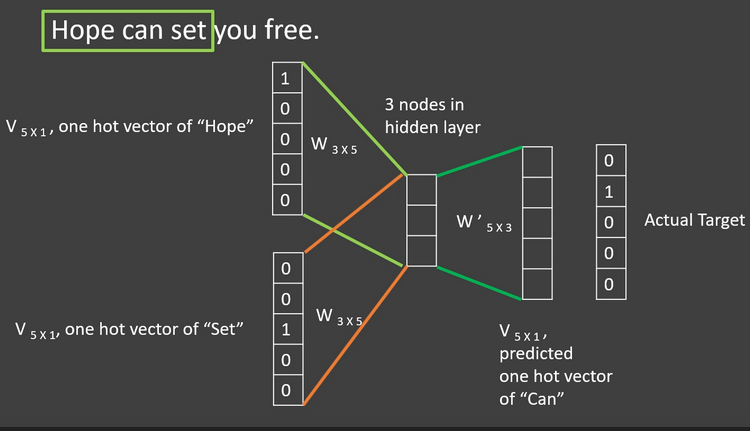
\includegraphics[width=0.8\textwidth]{cbow.png}
  \caption{CBOW}
  \label{fig:cbow}
\end{figure}
Passons sur un exemple concret traîté et expliqué dans la vidéo 
\cite[\textit{Word2Vec - Skip-gram and CBOW}, The Semicolon]{word2vec-semicolon}. 
Ici, notre corpus n'est que la phrase "Hope can set you free". On cherche à obtenir un word 
embedding de vecteurs à 3 dimensions, la couche cachée contient alors 3 neurones.

L'entrée 
contient un vecteur (dit \textit{hot} dans l'illustration) pour chaque mot de notre corpus. 
Ces vecteurs sont de dimension égale au nombre de mots dans le corpus. Dans cet exemple, cela 
donne des vecteurs de dimension 5. Pour représenter un mot à l'entrée, on remplit le vecteur 
de 0, à part la case qui correspond à la position du mot dans le corpus, qui sera mise à 1. 
On peut voir ceci sur l'image, même si dans l'image on ne voit que deux vecteurs d'entrée, 
on imagine qu'il y en a pour chaque mot du corpus. 

Pour la première itération, on prend le premier contexte de notre corpus. Dans cet exemple, 
on considère des contextes de taille 3, c'est-à-dire le voisin de gauche, le voisin de droite et le mot lui-même.
Notre contexte (notre entrée) est donc \textit{hope \_ set}, et on cherche à deviner le mot \textit{can}.
On multiplie les vecteurs d'entrée par une matrice W de dimension 3x5, pour passer à la couche cachée. 
On multiplie ensuite le vecteur de cette couche par une autre matrice W' de dimension 5x3 pour obtenir 
un vecteur de dimension 5 à la sortie. On compare ce vecteur au vecteur du mot qu'on cherche à deviner. 
Dans cet itération, c'est le mot \textit{can}, et donc son vecteur contient la valeur 1 dans sa deuxième 
case, car \textit{can} est le deuxième mot de notre corpus. Le résultat est donc comparé avec le vecteur 
du mot qu'on cherchait. On utilise ensuite des mathématiques des réseaux de neurones pour ajuster les 
valeurs dans les cases des matrices W et W'. On déplace le contexte à droite par un mot, et on recommence 
une autre itération. 
changer
Voici comment on récupère les vecteurs de nos mots à la fin de l'entraînement : la i-ème colonne de la 
matrice W correspondra au embedding (vecteur) du i-ème mot de notre contexte. 

\subsection{Alors pourquoi ça marche ?}
Le fait qu'un modèle si simple fonctionne si bien me paraissait magique au début. Si c'est le 
cas pour vous aussi, considérez la description suivante. 

A l'entrée, on a le contexte d'un mot donné. Par l'hypothèse distributionnelle, ceci code 
sa signification. On "comprime" cette information avec la matrice W pour passer à la couche 
cachée. On choisit la taille de la couche cachée pour correspondre à la dimensions des vecteurs 
qu'on veut obtenir. Ensuite, on "décomprime" cette information avec la matrice W' 
pour passer à la couche de sortie. 

Ce qui est essentiel, c'est qu'on ajoute une demande  
à cette "algo de compression", la demande étant qu'on veut que la couche de sortie 
correspond au mot donné au début (celui au milieu du contexte). La compression et la 
décompression sont donc obligées de garder la relation entre le contexte et le mot dans son 
milieu. Et comme cette relation représente la sémantique du mot, c'est la sémantique qui sera 
encodée dans ce processus. 

A la fin, on prend simplement "l'algo de compression" qu'on a utilisé, c'est-à-dire la matrice 
W comme notre word embedding. Cette "compression" est dans le format correcte (format qui 
correspond aux vecteurs qu'on veut), et elle encode la relation entre un mot et son contexte, 
ce qui est la sémantique (par l'hypothèse). Ce sont les qualités qu'on cherche dans un word 
embedding. 

Je me rends compte que cette description reste vague, mais je la trouve pas mal pour donner une
certaine explication ou "philosophie" intuitive à ce modèle. La raison précise pour la capacité de ces 
modèles à produire des word embeddings aussi bons n'est toujours pas connu, 
même s'il y a des articles qui essaie de s'y approcher. 

\subsection{Discussion}
\cite{wikipedia-wembedding} Le modèle Skip-gram est symétrique au CBOW. La seule différence étant qu'on prend un mot comme l'entrée, 
et on essaie de deviner son contexte dans le corpus. En général, le CBOW est plus rapide, et le 
Skip-gram a des meilleurs résultats sur des mots rares. Ces modèles 
seuls sont devenus dépassé, mais ils servent toujours comme un prétraitement pour les modèles 
d'apprentissage profond actuels, comme les transformeurs qui représentent actuellement l'état 
de l'art.  

\chapter{Conclusion}

\bibliographystyle{unsrt}
\bibliography{bibliographie}

\end{document}
